\input{preamble}

\begin{document}

\pagestyle{fancy}
\fancyhead[L]{Seconde}
\fancyhead[C]{\textbf{TD n°1 : rappels de collège}}
\fancyhead[R]{\today}

Les exercices les plus durs sont signalés par des étoiles.

\exe{, difficulty=0}{ 
Répondre par vrai ou faux, aucune justification n'est demandée.
\begin{enumerate}[label=(\alph*)]
\item $\dfrac13 = 0,333$
\item $\dfrac12 - \dfrac14 = \dfrac14$
\item $2x+1=3x$
\item $10^7 = \text{10 000 000}$
\item $2^4 = 2 \times 4$
\end{enumerate}
}{exe:exo1}{Les réponses sont, dans l'ordre : faux, vrai, faux, vrai et faux}

\exe{titre, difficulty=0}{
Effectuer les calculs ci-dessous sans calculatrice (donner les valeurs exactes).
\begin{multicols}{3}
\begin{enumerate}[label=(\alph*)]
	\item $\dfrac1{7} + \dfrac54$
	\item $\dfrac94 - \dfrac25$
	\item $\dfrac{11}4 \cdot 12$
	\item $\dfrac{10}3 \div 4$
	\item $\dfrac95 \cdot \dfrac{10}{27}$
	\item $\dfrac{\frac{25}{50}}{\frac{7}{28}}$
\end{enumerate}
\end{multicols}
}{exe:exo2}{
\begin{multicols}{3}
\begin{enumerate}[label=(\alph*)]
	\item $\dfrac1{7} + \dfrac54 = \dfrac{39}{28}$
	\item $\dfrac94 - \dfrac25 = \dfrac{37}{20}$
	\item $\dfrac{11}4 \cdot 12 = 33$
	\item $\dfrac{10}3 \div 4 = \dfrac56$
	\item $\dfrac95 \cdot \dfrac{10}{27} = \dfrac23$
	\item $\dfrac{\frac{25}{50}}{\frac{7}{28}} = 2$
\end{enumerate}
\end{multicols}
}

\exe{, difficulty=1}{
Dans cet exercice, $a, b, c$ et $d$ sont des entiers relatifs, avec $b \neq 0$ et $d \neq 0$.
\begin{enumerate}
\item Compléter la formule suivante $\frac{a}{b} + \frac{c}{d} = \mathord{?}$
\item Compléter la formule suivante $\frac{a}{b} \times \frac{c}{d} = \mathord{?}$
\item A quelle condition le nombre $a$ admet-il un inverse multiplicatif ? Si cet inverse existe, à quoi est-il égal ?
\item Compléter la formule suivante $\frac{a}{b} \div \frac{c}{d} = \mathord{?}$. Sous quelle condition cette formule est vraie ?
\item Compléter la formule ci-dessous :
\[ \dfrac{\frac{a}{b}}{\frac{c}{d}} = \mathord{?}  \]
Sous quelle condition cette formule est vraie ?
\end{enumerate}
}{exe:exo3}{
\begin{enumerate}
\item $\frac{a}{b} + \frac{c}{d} = \frac{ad+bc}{bd}$.
\item $\frac{a}{b} \times \frac{c}{d} = \frac{ac}{bd}$.
\item tout réel non nul admet un inverse multiplicatif et si $a \neq 0$ alors $a^{-1}=\frac1{a}$.
\item si $c \neq 0$ alors $\frac{a}{b} \div \frac{c}{d} = \frac{ad}{bc}$.
\item si $c \neq 0$ alors
\[ \dfrac{\frac{a}{b}}{\frac{c}{d}} = \dfrac{ad}{bc} . \]
\end{enumerate}
}

\exe{, difficulty=1}{
\begin{enumerate}
\item Rappeler la définition de $a^n$ pour $a \in \Z$ et $n \in \N$.
\item Expliciter la règle de calcul ci-dessous :
\[ a^n \times b^m = \mathord{?} \qquad \text{ avec } a, b \in \Z \text{ et } n, m \in \N . \]
\item Rappeler la définition de $a^{-1}$ pour $a \in \Z$.
\item En déduire la définition de $a^{-n}$ pour $a \in \Z$ et $n \in \N$.
\item Expliciter la règle de calcul ci-dessous :
\[ \frac{a^n}{b^m} = \mathord{?} \qquad \text{ avec } a, b \in \Z \text{ et } n, m \in \N . \]
\end{enumerate}
}{exe:exo4}{
\begin{enumerate}
\item Pour $a \in \Z$ et $n \in \N, a^n=\underbrace{a \times a \times \dots a}_{\text{n fois}}$
\item Pour $a, b \in \Z$ et $n, m \in \N$ :
\[ a^n \times b^m = \underbrace{a \times a \times \dots a}_{\text{n fois}} \times \underbrace{b \times b \times \dots b}_{\text{m fois}} \] 
En particulier, si $a=b$ :
\[ a^n \times a^m = \underbrace{a \times a \times \dots a}_{\text{n+m fois}} = a^{n+m}. \]
\item Pour $a \in \Z$, si $a \neq 0, a^{-1}=\frac{1}{a}$.
\item Pour $a \in \Z$ et $n \in \N, a^{-n} = \underbrace{\frac{1}{a \times a \times \dots \times a}}_{\text{n fois}}$
\item Pour $a, b \in \Z$ et $n, m \in \N$ :
\[ \frac{a^n}{b^m} = \dfrac{\underbrace{a \times a \times \dots a}_{\text{n fois}}}{\underbrace{b \times b \times \dots b}_{\text{m fois}}}\]
En particulier, si $a=b$ :
\[ a^n \times b^m = \dfrac{\underbrace{a \times a \times \dots a}_{\text{n fois}}}{\underbrace{a \times a \times \dots a}_{\text{m fois}}} = a^{n-m}. \]
\end{enumerate}
}

\exe{, difficulty=0}{
Résoudre pour $x$ les équations suivantes (donner l'ensemble des solutions).
\begin{multicols}{3}
\begin{enumerate}[label=(\alph*)]
	\item $2x+3=5$
	\item $7x - 5=4$
	\item $11x + 15 = 2$ 
	\item $\dfrac{10}3 x + 8 = \dfrac14 x + 1$
	\item $(5x-3)(7x+2)=0$
	\item $x \neq 0, \frac{1}{x} + 2 = 6$ 
\end{enumerate}
\end{multicols}
}{exe:exo5}{
\begin{multicols}{3}
\begin{enumerate}[label=(\alph*)]
	\item $x=1$
	\item $x=\frac{9}{7}$
	\item $x=-\frac{13}{11}$ 
	\item $x=-\frac{84}{43}$
	\item $x=\frac35$ ou $x=-\frac27$
	\item $x=\frac14$ 
\end{enumerate}
\end{multicols}
}

\exe{, difficulty=1}{
Résoudre pour $x$ les inéquations suivantes (donner l'ensemble des solutions).
\begin{multicols}{2}
\begin{enumerate}[label=(\alph*)]
	\item $7x - 3 > 2x - 1$
	\item $-3x -8 \leq x-1$
	\item $2 \cdot (x+5) > (x+3) - (x-1)$
	\item $5x \leq 5x-2$
\end{enumerate}
\end{multicols}
}{exe:exo6}{
\begin{multicols}{2}
\begin{enumerate}[label=(\alph*)]
	\item $7x - 3 > 2x - 1 \equi 5x > 2 \equi x > \frac25$
	\item $-3x -8 \leq x-1 \equi -7 \leq 4x \equi \frac{-7}4 \leq x$
	\item $2 \cdot (x+5) > (x+3) - (x-1) \equi x > -3$
	\item $5x \leq 5x-2 \equi 0 \leq -2$ c'est impossible ! Aucune valeur ne convient.
\end{enumerate}
\end{multicols}
}

\exe{, difficulty=0}{
On considère la fonction $f$ définie sur $\R$ par $f(x)=5x-7$.
\begin{enumerate}
	\item Déterminer l'image de $0$ par la fonction $f$.
	\item Déterminer, s'il existe, l'antécédent de $0$ par la fonction $f$.
	\item Représenter la fonction $f$ dans un repère orthonormé.
	\item On définit la fonction $g$ par $g(x) = \left \{ \begin{array}{c c c} f(x) & \qquad & \text{ si } x <0 \\ 0 & \qquad & \text{sinon} \end{array} \right.$
	\begin{enumerate}
		\item Représenter la fonction $g$ dans le repère déjà construit.
		\item Déterminer, s'il existe, l'antécédent de $1$ par la fonction $g$.
	\end{enumerate}
\end{enumerate}
}{exe:exo7}{
\begin{enumerate}
	\item $f(0)=5 \times 0 - 7 = -7$.
	\item On cherche $x$ tel que $f(x)=0 \equi 5x-7=0 \equi x = \frac75$.
	\item 
	\begin{enumerate}
		\item Les représentations de $f$ et $g$ sont données ci-dessous. A noter que $f(x)=g(x)$ pour $x<0$. 
		\begin{center}
		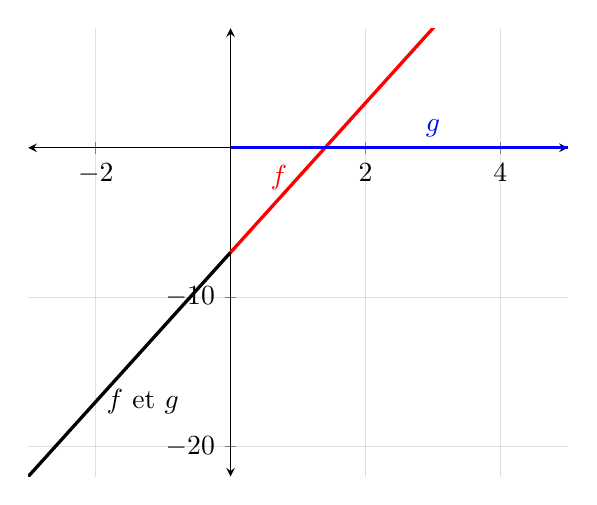
\begin{tikzpicture}[>=stealth, scale=1]
			\begin{axis}[xmin = -3, xmax= 5, ymin=-22, ymax=8, axis x line=middle, axis y line=middle, axis line style=<->,
			xlabel={}, ylabel={}, grid=both, grid style = {opacity=.5}]]
			\addplot[black, very thick, domain =-3:-2, samples=2] {5*x-7}  node[right] {$f$ et $g$};
			\addplot[black, very thick, domain =-2:0, samples=2] {5*x-7} ;
			\addplot[red, very thick, domain =0:1, samples=2] {5*x-7}  node[left] {$f$};
			\addplot[red, very thick, domain = 1:5, samples=2] {5*x-7} ;
			\addplot [blue, very thick, domain = 0:3, samples=2]{0} node[above] {$g$};
			\addplot [blue, very thick, domain = 3:5, samples=2]{0} ;
			\end{axis}
		\end{tikzpicture}
		\end{center}
		\item On remarque que $g(x) < 0$ pour $x<0$ et $g(x)=0$ pour $x \geq 0$, il n'existe donc pas de $x \in \R$ tel que $g(x)=1$.
	\end{enumerate}
\end{enumerate}
}

\exe{Racine carrée, difficulty=0}{
\begin{enumerate}
	\item Résoudre pour $x$ l'équation $x^2 = 2$. Comment s'appelle l'outil mathématique utilisé ?
	\item Les valeurs trouvées à la question précédente sont-elles entières ?
	\item Même question pour $x^2 = 144$.
\end{enumerate}
}{exe:exo8}{
\begin{enumerate}
	\item $x^2 = 2 \equi x = \pm \sqrt{2}$ (attention, il y a deux solutions !). L'outil s'appelle ``racine carrée''.
	\item Non, ces valeurs ne sont pas entières. On propose une démonstration. On remarque d'abord que si $x \leq y$ alors $x^2 \leq y^2$. Supposons que $\sqrt(2) \leq 1$, alors $2 \leq 1$, ce qui est absurde. Supposons que $2 \leq \sqrt{2}$, alors $4 \leq 2$ ce qui est aussi absurde. Finalement, $1 < \sqrt{2}<2$ (à noter les inégalités \textbf{strictes}).
	\item $x^2 = 144 \equi x = \pm 12$. Cette fois les solutions sont entières. C'est toujours le cas pour une équation de la forme $x^2 = k$ avec $k$ un carré parfait.
\end{enumerate}
}

\exe{titre=Notation scientifique, difficulty=0}{
\begin{enumerate}
\item Rappeler la définition de la notation scientifique d'un nombre.
\item Sans calculatrice, écrire les nombres suivants en notation scientifique :
	\begin{multicols}{3}
	\begin{enumerate}
		\item 201
		\item 10
		\item 123 400 000
		\item 0,8
		\item 0,000 327
		\item 0,009 000 1
	\end{enumerate}
	\end{multicols}
\end{enumerate}
}{exe:exo9}{
\begin{enumerate}
\item Soit $x \in \R$, on appelle notation scientifique de $x$ son écriture sous la forme :
\[ x = \pm a \cdot 10^n \]
avec $a$ un réel de l'intervalle $[0, 10[$ (i.e. $0 \leq a < 10$) et $n \in \Z$.
	\begin{multicols}{3}
	\begin{enumerate}
		\item $201=2,01 \cdot 10^2$
		\item $10=1,0 \cdot 10^1$
		\item $123~400~000 = 1,234 \cdot 10^8$
		\item $0,8 = 8 \cdot 10^{-1}$
		\item $0,000~327 = 3,27 \cdot 10^{-4}$
		\item $0,009~000~1 = 9,000~1 \cdot 10^{-3}$
	\end{enumerate}
	\end{multicols}
\end{enumerate}
}

\exe{, difficulty=2}{
On considère les fonctions $f$ et $g$ définies sur $\R$ par $f(x)=2x-1$ et $g(x)=(x-1)^2$.
\begin{enumerate}
	\item Représenter les fonctions $f$ et $g$ dans un même repère orthonormé. Les courbes tracées se croisent-elles ? En combien de points ?
	\item Déterminer les coordonnées des éventuels points d'intersection des courbes représentatives de $f$ et $g$.
	\item On remplace l'expression de la fonction $f$ par $f(x)=ax+b$ avec $a, b$ des réels quelconques. Est-ce que les courbes représentatives de $f$ et de $g$ présentent \textbf{toujours} un point d'intersection (c-à-d quelles que soient les valeurs de $a$ et $b$) ? Justifier. 
\end{enumerate}
}{exe:exo10}{Correction non fournie (exercice de recherche)}

\newpage
\fancyhead[C]{\textbf{Solutions}}
\shipoutAnswer

\end{document}